% called by main.tex
%
\chapter{Resultados y análisis}
\label{ch::resultados}

Este capítulo separa dos niveles de evidencia que no deben confundirse. Primero se presenta
la evaluación confirmatoria del especialista base, congelado antes de observar el bloque del
6 al 10 de junio. Después se documenta el diagnóstico de volatilidad realizado sobre ese mismo
bloque. El segundo resultado es útil para formular una política futura, pero no constituye
una nueva validación fuera de muestra.

\section{Resultados obtenidos}

\subsection{Validación fuera de muestra del especialista base}

El especialista congelado selecciona 754 unidades de acción en los cinco días fuera de
muestra. Sin aplicar ningún filtro decidido a partir de esos datos, obtiene un neto medio de
$+0{,}349$ ticks al coste de referencia. El promedio es positivo en tres de cinco días y
pasa a ser ligeramente negativo ($-0{,}026$ ticks) cuando se carga el coste visible completo
(Tabla~\ref{tab:fresh}). Esta es la estimación limpia del rendimiento fuera de muestra.

\begin{table}[h]
\centering
\caption{Validación fuera de muestra del especialista base congelado. Los valores son ticks
netos por unidad de acción y no incorporan el filtro de volatilidad posterior.}
\label{tab:fresh}
\begin{tabular}{lr}
\toprule
\textbf{Métrica} & \textbf{Valor} \\
\midrule
Unidades de acción ($n$)                  & 754 \\
Días de soporte                          & 5 (3/5 positivos) \\
Neto medio (coste 0,25, optimista)         & $+0{,}537$ ticks \\
Neto medio (coste 0,5, referencia)         & $+0{,}349$ ticks \\
Neto medio (coste 1,0, estrés)             & $-0{,}026$ ticks \\
\bottomrule
\end{tabular}
\end{table}

\begin{table}[h]
\centering
\caption{Desglose diario del especialista base al coste de referencia.}
\label{tab:base_daily}
\begin{tabular}{lrr}
\toprule
\textbf{Día} & \textbf{$n$} & \textbf{Neto medio @0,5} \\
\midrule
6 de junio  & 220 & $+0{,}666$ \\
7 de junio  &  97 & $+1{,}342$ \\
8 de junio  & 241 & $+0{,}308$ \\
9 de junio  & 146 & $-0{,}565$ \\
10 de junio &  50 & $-0{,}105$ \\
\bottomrule
\end{tabular}
\end{table}

El signo positivo al coste de referencia indica que el especialista conserva una señal
modesta donde los modelos anteriores habían fracasado. Sin embargo, ni la estabilidad diaria
ni el escenario de coste completo permiten calificarlo como una política robusta. La lectura
defendible es, por tanto, \emph{señal parcial fuera de muestra}, no rentabilidad demostrada.

\subsection{Diagnóstico \emph{post-hoc} del régimen de volatilidad}

La inspección del bloque reveló que la fracción de sesiones de alta volatilidad aumentó hasta
aproximadamente el 58\,\%, frente al 18--22\,\% de los periodos históricos
(Figura~\ref{fig:regimen}). Para estudiar ese desplazamiento se dividió la selección con el
umbral 0,6657, percentil 80 de la volatilidad de entrenamiento. El umbral numérico no se
ajustó al bloque nuevo, pero la decisión de usarlo como filtro sí se tomó tras observarlo; por
ello, todo lo que sigue en esta subsección es diagnóstico y exploratorio.

\begin{figure}[h]
\centering
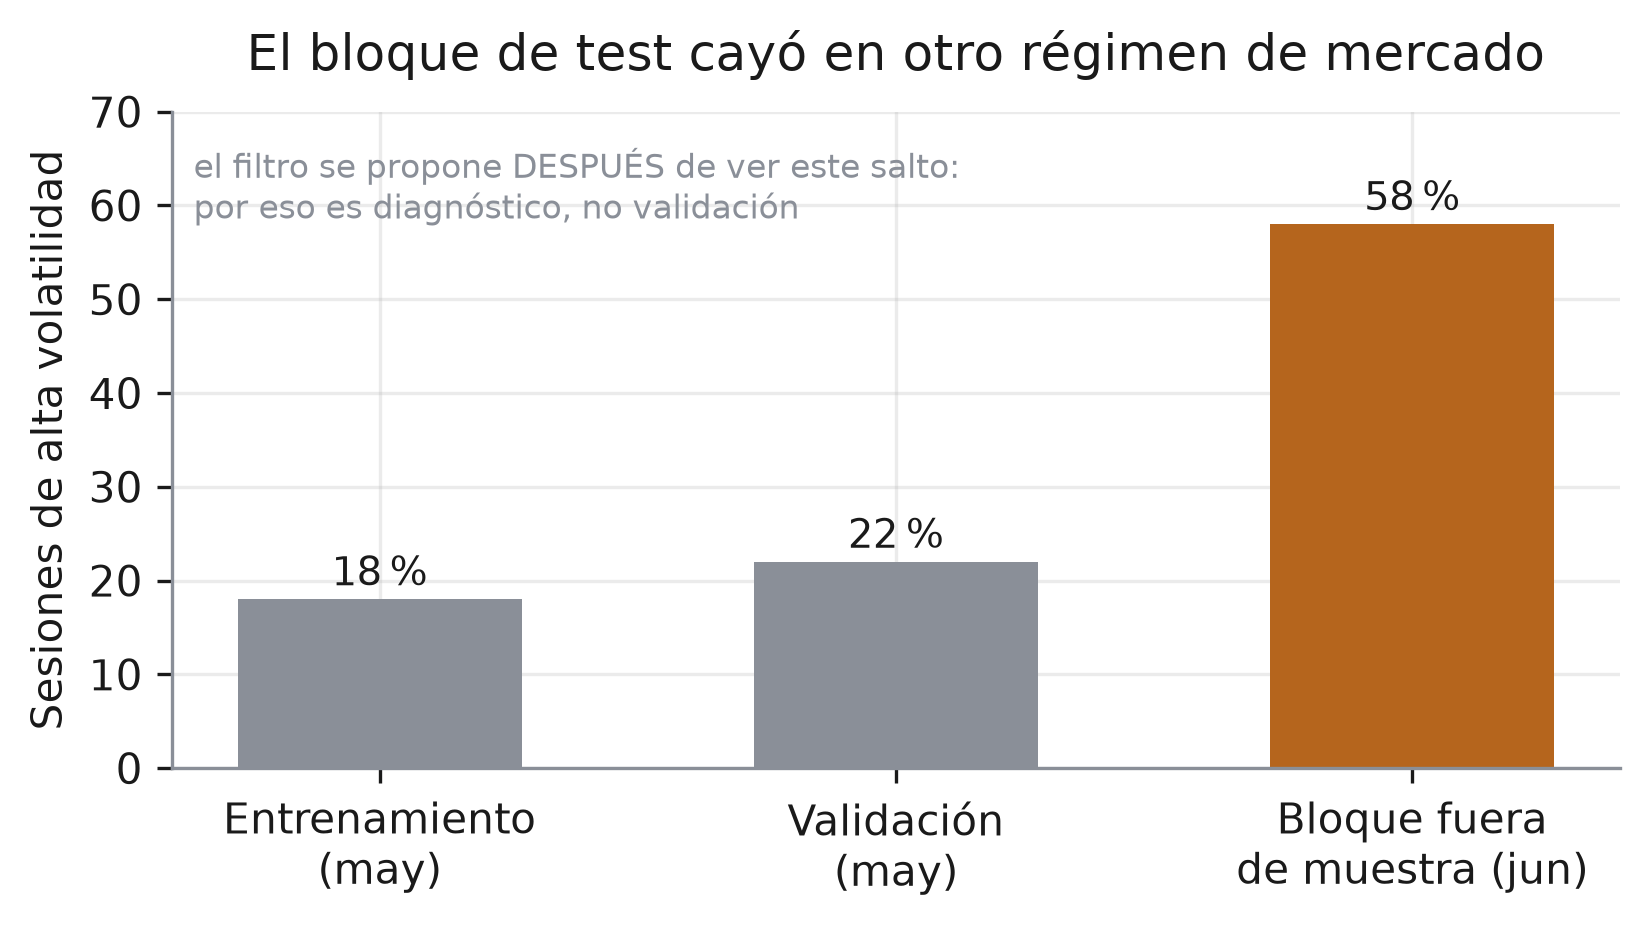
\includegraphics[width=0.6\textwidth]{figures/fig_regimen.png}
\caption{Fracción de sesiones de alta volatilidad por periodo. El salto del bloque nuevo
motiva el análisis de régimen, pero no valida por sí mismo el filtro.}
\label{fig:regimen}
\end{figure}

La Tabla~\ref{tab:regimen} muestra el contraste. Hay 318 acciones de baja volatilidad, 435 de
alta volatilidad y una acción sin dato de volatilidad, que una regla operativa conservadora
rechazaría. Las primeras son positivas y las segundas, negativas al coste de referencia.

\begin{table}[h]
\centering
\caption{Diagnóstico \emph{post-hoc} por régimen en el bloque del 6--10 de junio (ticks por
unidad de acción).}
\label{tab:regimen}
\begin{tabular}{lrrrr}
\toprule
\textbf{Régimen} & \textbf{$n$} & \textbf{@0,25} & \textbf{@0,5} & \textbf{@1,0} \\
\midrule
Baja volatilidad   & 318 & $+1{,}258$ & $+1{,}069$ & $+0{,}691$ \\
Alta volatilidad   & 435 & $+0{,}004$ & $-0{,}183$ & $-0{,}558$ \\
Volatilidad ausente&   1 & $+3{,}327$ & $+3{,}154$ & $+2{,}807$ \\
\midrule
Total sin filtro   & 754 & $+0{,}537$ & $+0{,}349$ & $-0{,}026$ \\
\bottomrule
\end{tabular}
\end{table}

\begin{figure}[h]
\centering
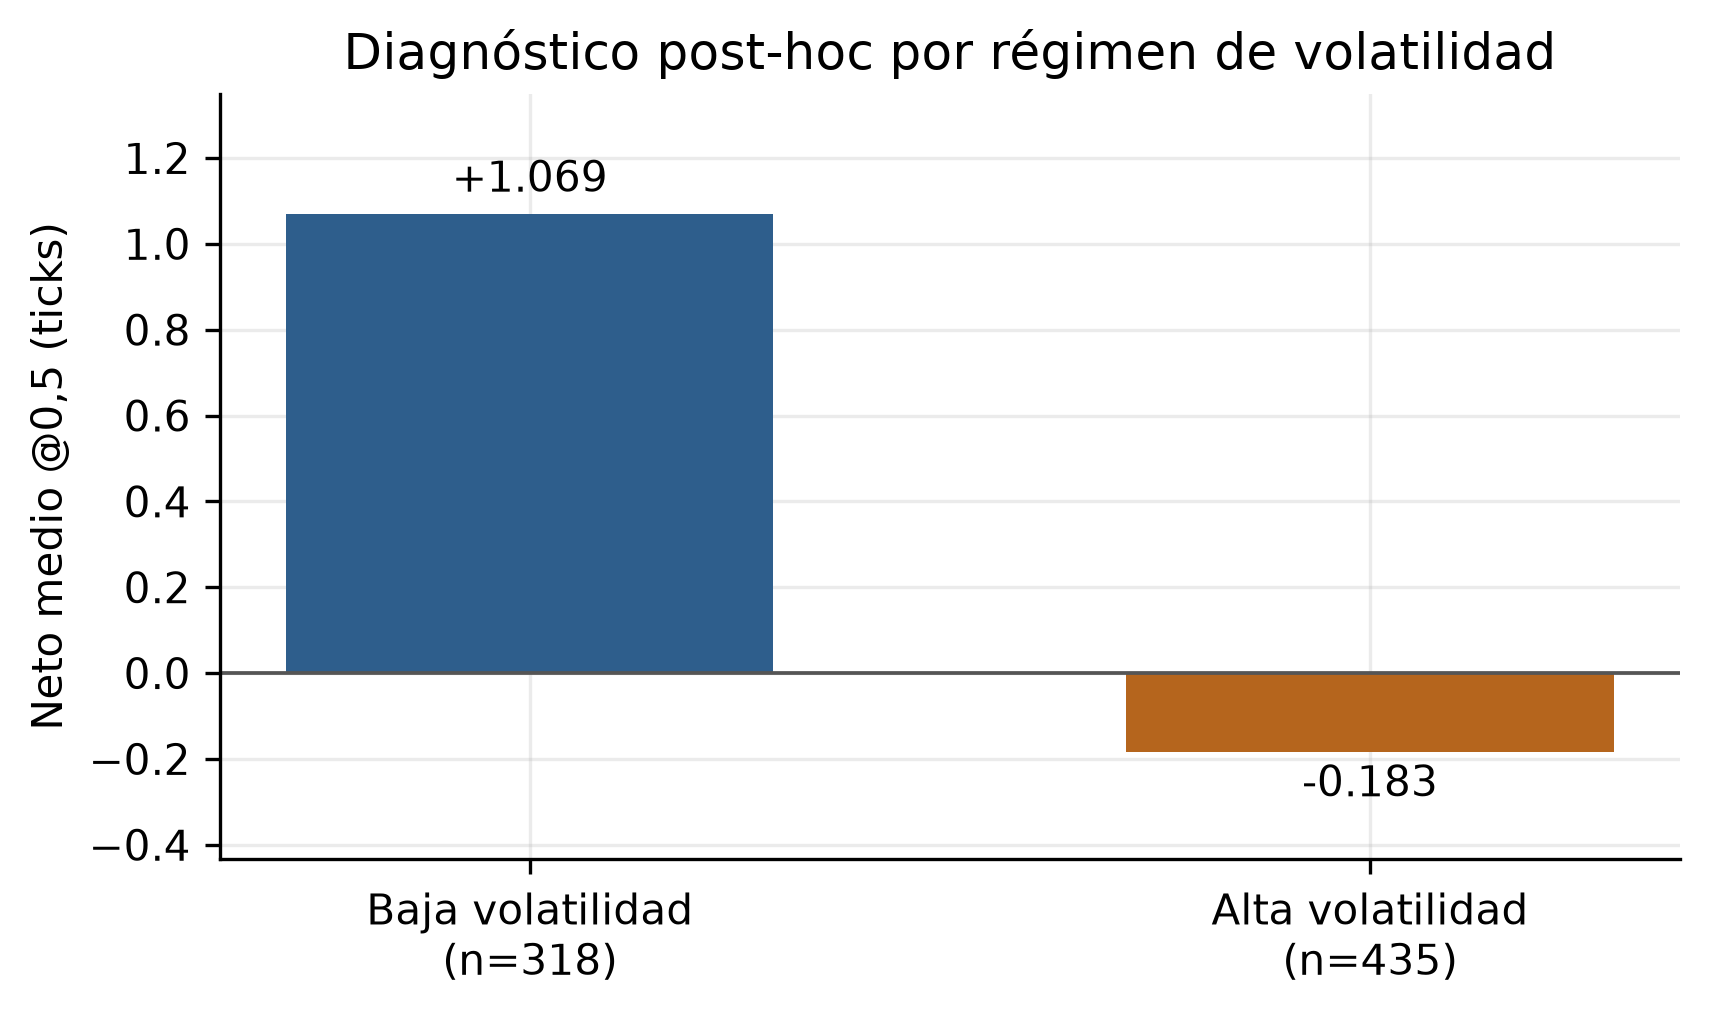
\includegraphics[width=0.56\textwidth]{figures/fig_regimen_neto.png}
\caption{Contraste \emph{post-hoc} del neto medio entre baja y alta volatilidad. La separación
es una hipótesis de política que requiere datos posteriores.}
\label{fig:regimenneto}
\end{figure}

Si se aplica retrospectivamente el filtro de baja volatilidad, el subconjunto de 318 acciones
mantiene signo positivo en los tres niveles de coste (Figura~\ref{fig:coste}) y en los cinco
días (Figura~\ref{fig:netodiario}). Su suma cronológica presenta un drawdown diagnóstico de
88,1 ticks (Figura~\ref{fig:drawdown}). Estas magnitudes describen el subconjunto observado;
no son PnL de una cartera ejecutada.

\begin{figure}[h]
\centering
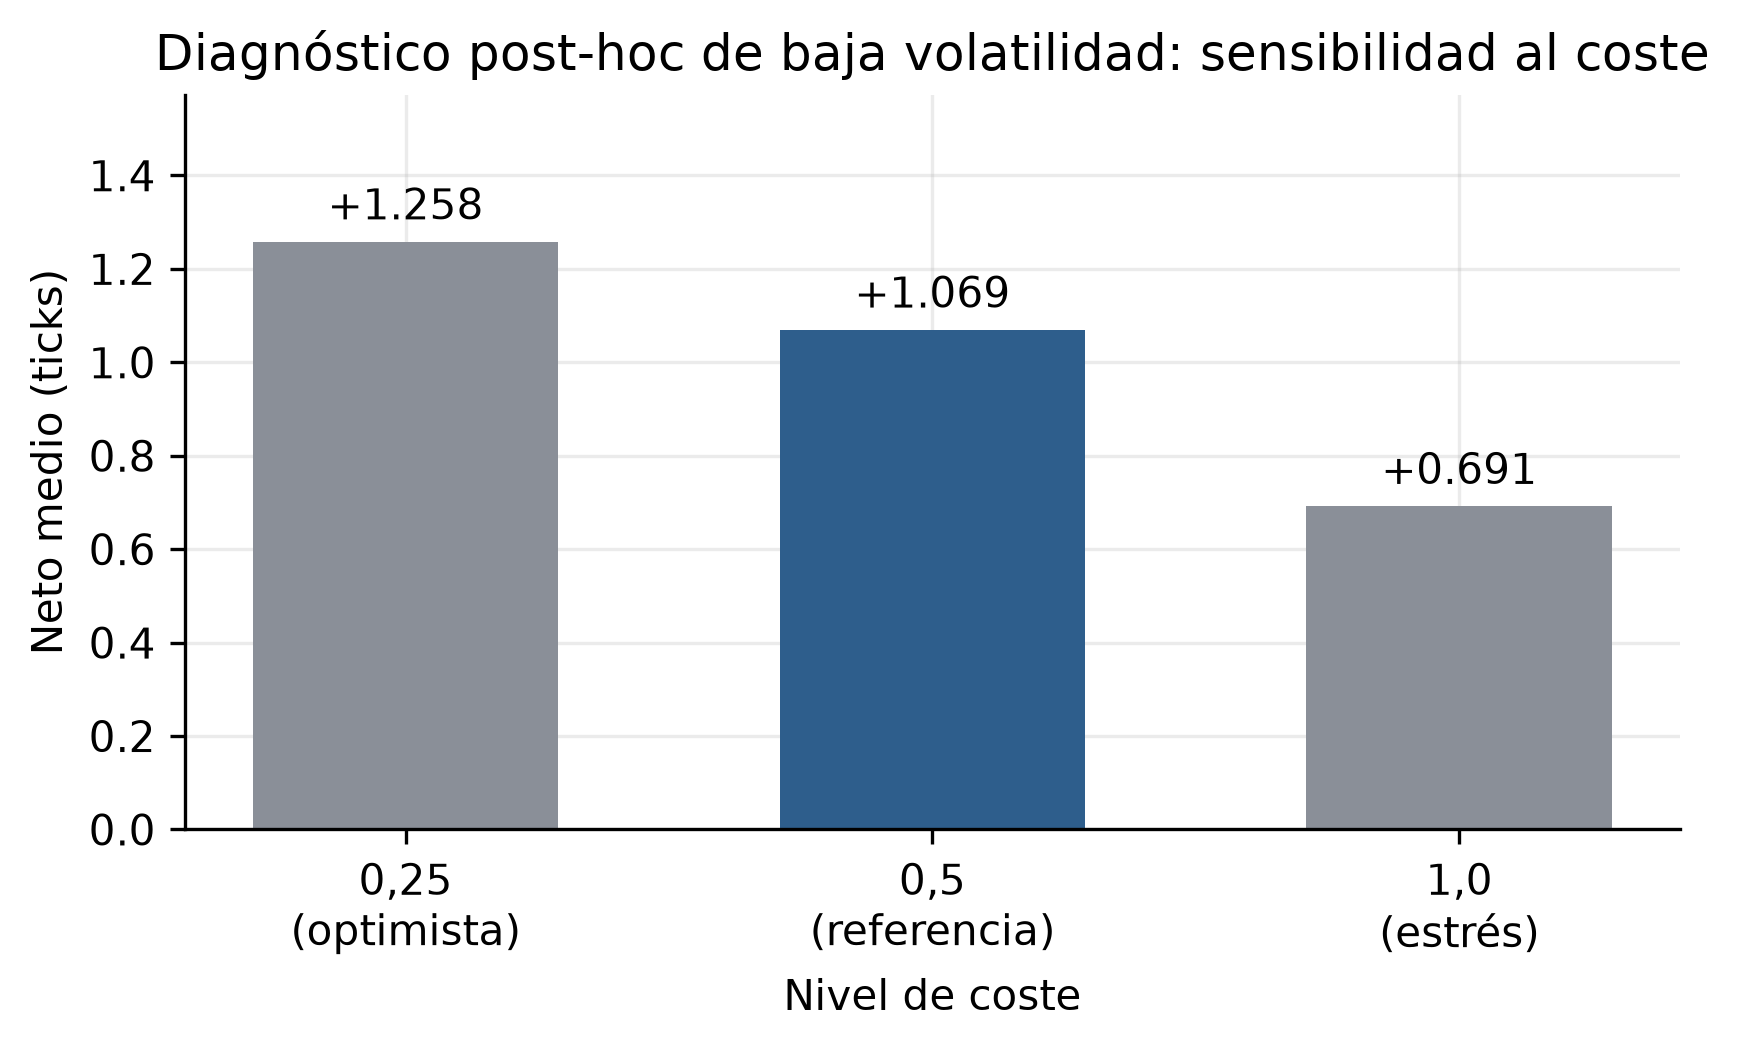
\includegraphics[width=0.55\textwidth]{figures/fig_coste.png}
\caption{Sensibilidad al coste del subconjunto de baja volatilidad. Resultado exploratorio
obtenido tras inspeccionar el mismo bloque.}
\label{fig:coste}
\end{figure}

\begin{figure}[h]
\centering
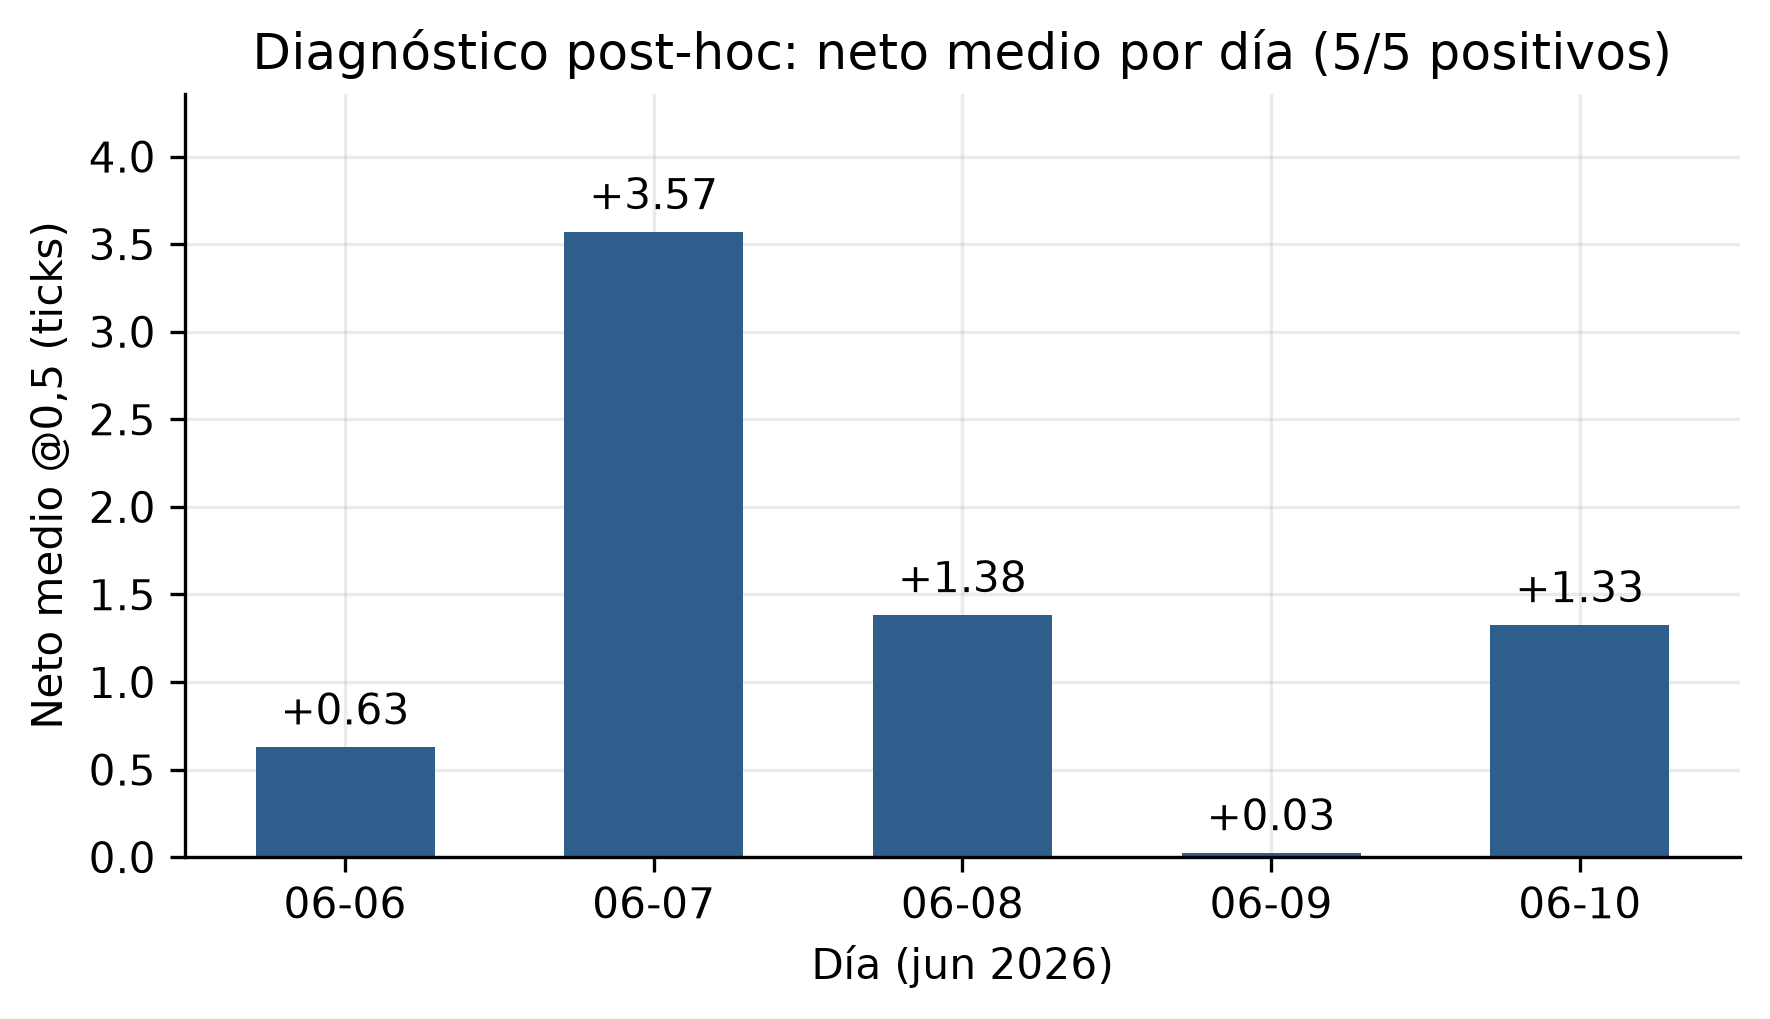
\includegraphics[width=0.62\textwidth]{figures/fig_neto_diario.png}
\caption{Neto medio diario del subconjunto \emph{post-hoc} de baja volatilidad.}
\label{fig:netodiario}
\end{figure}

\begin{figure}[h]
\centering
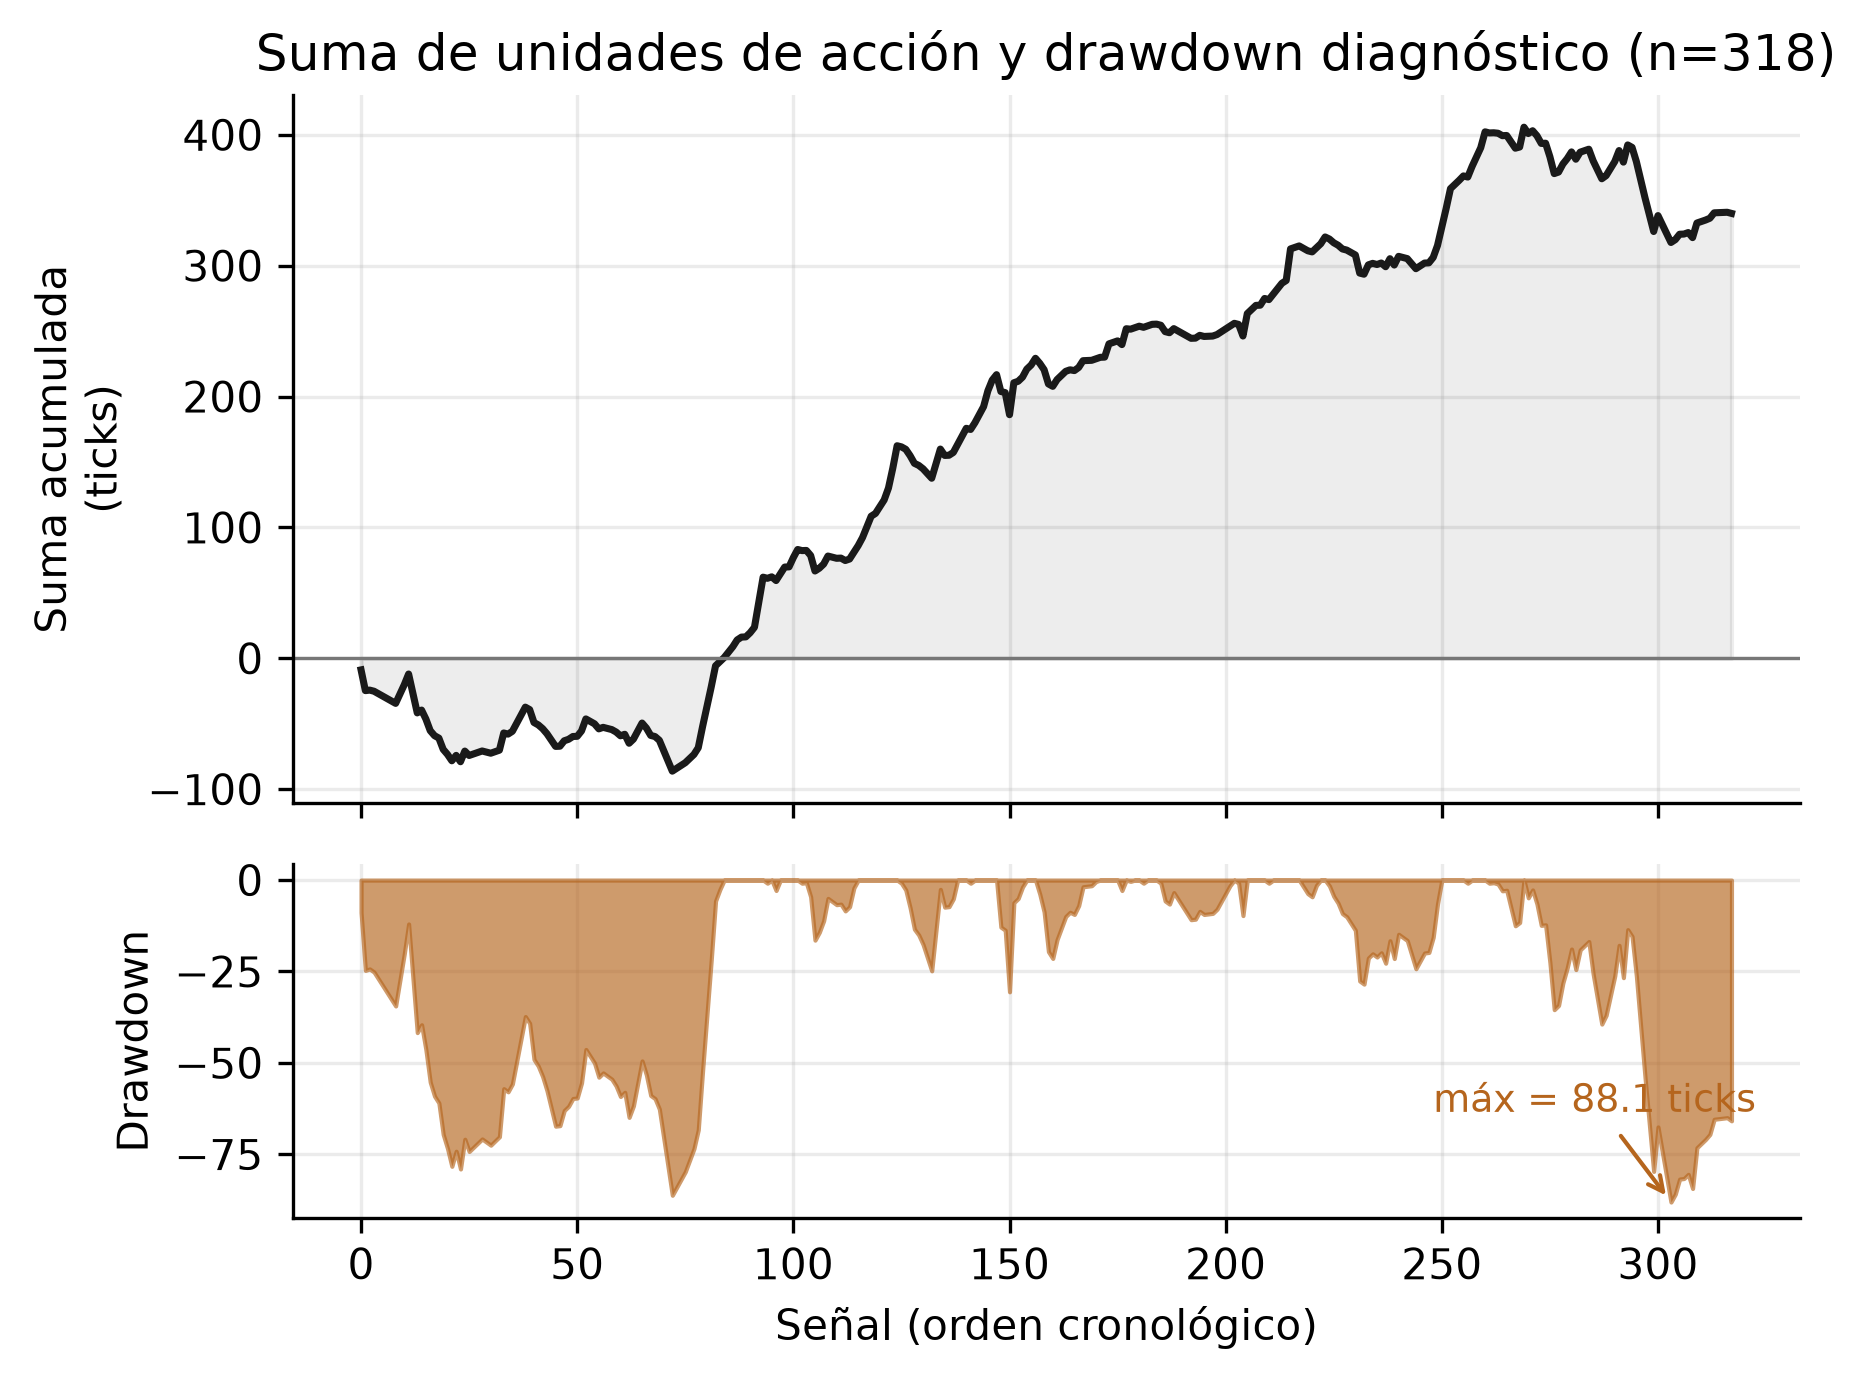
\includegraphics[width=0.62\textwidth]{figures/fig_drawdown.png}
\caption{Suma acumulada y drawdown diagnóstico de 318 unidades de acción. No representa una
cartera con restricciones de capital o de exposición simultánea.}
\label{fig:drawdown}
\end{figure}

El remuestreo independiente de las 318 acciones produce un IC90 de
$[+0{,}472,+1{,}654]$ y $P=0{,}998$, pero esa estimación ignora la dependencia entre señales
del mismo mercado. Hay 156 mercados y hasta ocho acciones por mercado. Un \emph{bootstrap}
agrupado por mercado amplía el IC90 a $[+0{,}193,+2{,}004]$ y reduce la probabilidad estimada
a 97,6~\%. Ambos cálculos son descriptivos: la selección \emph{post-hoc} impide darles una
lectura confirmatoria.

\subsection{Registro de sombra retrospectivo}

Para auditar la mecánica de la política candidata se construyó un registro de sombra
\emph{offline}: conserva cada unidad de acción, su mercado, el resumen diario y las reglas de
promoción. Es una reproducción retrospectiva de lo que la regla habría indicado, no una
ejecución prospectiva ni un sistema activo en tiempo real. El filtro queda congelado después
del 10 de junio; solo observaciones posteriores pueden contar para las puertas de promoción.

Además, varias señales pertenecen al mismo mercado y sus horizontes H60 se solapan. Por ello
se denominan \emph{unidades de acción}, no operaciones independientes, y la suma acumulada no
incorpora una regla de exposición máxima. Una futura sombra prospectiva deberá decidir si
permite apilar posiciones o admite una sola posición por mercado.

\subsection{Resultados con la comisión oficial de 2026 (capa taker-real)}
\label{sec::taker_real}

La corrección del modelo de costes (Sección~\ref{sec::fe_erratas_fees}) obliga a
re-evaluar la política congelada con la comisión oficial de 2026. La operación se hizo sin
reentrenar nada: los mismos artefactos sellados, la misma selección de acciones, y como
control de integridad se reprodujeron primero las cifras publicadas (la política
\texttt{ev>0{,}75, healthy\(\ge\)0{,}5} da $n=754$ y $+0{,}349$ ticks netos al coste de
referencia; el corte de baja volatilidad, $n=318$ y $+1{,}069$). Después se aplicó la
comisión real. La Tabla~\ref{tab::taker_real} resume el resultado.

\begin{table}[htbp]
\centering
\caption{Política congelada re-evaluada con la comisión oficial de 2026. Ticks netos
medios por acción; «solo entrada» es la cota optimista que omite la comisión de salida,
«ida y vuelta» carga ambas. Las comisiones medias medidas son de 1,75 ticks a la entrada
y 1,71 a la salida.}
\label{tab::taker_real}
\begin{tabular}{lccc}
\toprule
 & & \multicolumn{2}{c}{Fee oficial 2026} \\
\cmidrule(lr){3-4}
Corte & Publicado (fee errónea) & solo entrada & ida y vuelta \\
\midrule
Todas las acciones ($n=754$) & $+0{,}349$ & $-1{,}059$ & $-3{,}304$ \\
Baja volatilidad ($n=318$) & $+1{,}069$ & $-0{,}342$ & $-2{,}604$ \\
\bottomrule
\end{tabular}
\end{table}

El resultado es inequívoco: \emph{ningún corte taker es positivo} bajo el régimen de
comisiones vigente, ni siquiera en la cota optimista que solo carga la comisión de
entrada. La comisión media de entrada (1,75 ticks) supera por sí sola el resultado bruto
de la señal. Este número negativo no es un fracaso del trabajo, sino su lección central
confirmada estructuralmente: una precisión direccional cercana al 90\,\% —demostrada en
los capítulos anteriores— no se traduce en beneficio cuando el coste de ejecución la
domina. «Acertar no es ganar» deja de ser una advertencia metodológica y pasa a ser una
consecuencia medida del régimen de comisiones. La política congelada se reporta, por
tanto, tal cual: negativa en la capa taker, lo que motiva el giro al lado maker del
Capítulo~\ref{ch::despliegue} y no una búsqueda de umbrales que la rescaten.

\subsection{Validación prospectiva pre-registrada}
\label{sec::validacion_prospectiva}

Todo lo anterior en este capítulo comparte una debilidad que ninguna técnica estadística
puede reparar: se mide sobre datos que ya existían cuando se diseñó la política. Por
cuidadosa que sea la separación entre entrenamiento y prueba, el analista ha visto el
periodo, ha iterado sobre él y ha tomado decisiones informadas por lo que allí ocurría. La
única refutación limpia de esa objeción es evaluar sobre datos que todavía no existían
cuando la política quedó congelada. Esta sección recoge esa evaluación.

\subsubsection{Cadena de compromiso}

El procedimiento se diseñó para que el autor no pudiera ajustarlo después de ver los
resultados, y para que un tercero pueda comprobarlo sin tener que fiarse de su palabra.
Antes de que existiera un solo día de la ventana, se fijaron por escrito y se sellaron:
el universo de mercados, los filtros, la configuración exacta del simulador, los brazos
que se ejecutarían, las métricas que se reportarían y las reglas de decisión, junto con
las huellas criptográficas de los cinco artefactos ejecutables. El documento se registró
además en la cadena de bloques de Bitcoin mediante OpenTimestamps~\cite{opentimestamps},
de modo que su fecha es verificable con independencia del repositorio y del autor. El
Anexo~\ref{anexo:preregistro} reproduce el pre-registro y el procedimiento de
verificación del sello.

La cadena tiene una divergencia deliberada que conviene declarar aquí y no en una nota al
pie: la huella del motor de simulación que consta en el pre-registro no es la del motor
que se ejecutó. El 13 de julio de 2026 se detectó y corrigió una errata que impedía
ejecutar el brazo base, y la corrección se selló a su vez con su propia marca de tiempo.
Revertir al artefacto originalmente sellado no habría hecho el experimento más honesto:
lo habría hecho imposible, porque el brazo de referencia no llegaba a completar una
corrida. Se conserva por tanto la cadena completa —sello original, errata, sello de la
errata— y se reporta la divergencia como parte del resultado.

\subsubsection{Ventana de evaluación}

La ventana comprende \textbf{35~días completos, del 10 de julio al 13 de agosto de 2026},
ambos incluidos. Su comienzo está determinado por el pre-registro, que excluye
explícitamente los días 6 a 9 de julio por haberse empleado en el desarrollo del
simulador. Su final no lo decidió el autor: el 14 de agosto la captura se interrumpió por
una desconexión física del almacenamiento del recolector, descrita en el
Capítulo~\ref{ch::etica}. El último día íntegro es el 13 de agosto.

Esa circunstancia, que operativamente fue un contratiempo, refuerza metodológicamente el
resultado. La objeción más natural a cualquier evaluación prospectiva es que el analista
elija cuándo parar, y que esa elección dependa de lo que va viendo. Aquí el punto de corte
lo fijó un fallo de hardware tres días antes de que se ejecutara la primera evaluación, y
la cobertura se verificó sobre el registro de sesiones del recolector —unas 225 sesiones
diarias, sin un solo día incompleto dentro de la ventana— antes de calcular ninguna
métrica de resultado. El mínimo declarado en el pre-registro era de 25~días evaluados; la
ventana disponible lo supera en un 40\,\%.

\subsubsection{Brazos y capas}

Se ejecutan los \textbf{tres brazos declarados}, y los tres se reportan con independencia
de su signo. El brazo \emph{base} es la configuración congelada operando sin señal. El
brazo \emph{suppress\_ask} suprime durante 240~segundos la cotización de venta del token
favorecido por la señal H60. El brazo \emph{tight\_risk} activa, en los mercados
señalados, un régimen de riesgo estricto que reduce a la mitad el límite de inventario y
el sesgo de inventario y duplica el número de fotogramas en plano. La partición por el
gate de regímenes congelado descrito en la Sección~\ref{sec::brazos_gate} se reporta como
análisis secundario, con su hipótesis registrada de antemano.

Las métricas son las del pre-registro, sin añadidos: equity neta —caja más inventario
valorado a resolución más \emph{rebates}—, su descomposición en las tres partidas,
\emph{markout} a corto plazo, peor día y porcentaje de mercados con resultado positivo.

\subsubsection{Reglas de decisión, declaradas antes de mirar}

La Tabla~\ref{tab::puertas_b3} recoge las tres condiciones que el pre-registro declara
para promover la política a operación en sombra, y la regla de sustitución entre brazos.
Se rellenan y se obedecen sin interpretación. Conviene subrayar que un resultado negativo
no es un fracaso del trabajo ni obliga a reescribir nada: el pre-registro declara
explícitamente que el experimento es informativo en cualquier dirección y que todo corte
se reporta completo. La contribución de esta sección es el procedimiento y su ejecución
honesta, no el signo del número que produzca.

\begin{table}[htbp]
\centering
\caption[Puertas de decisión pre-declaradas]{Puertas de decisión pre-declaradas para el
corte prospectivo nº~1, sobre el brazo base. Las tres condiciones deben cumplirse
simultáneamente.}
\label{tab::puertas_b3}
\begin{tabular}{lcc}
\hline
\textbf{Condición} & \textbf{Valor medido} & \textbf{¿Cumple?} \\
\hline
Equity neta $> 0$ & --- & --- \\
Peor día $> -150$\,\$ simulados & --- & --- \\
Días evaluados $\geq 25$ & 35 & Sí \\
\hline
\end{tabular}
\end{table}

\begin{table}[htbp]
\centering
\caption[Resultado del corte prospectivo por brazo]{Resultado del corte prospectivo
nº~1 por brazo, con la descomposición declarada en el pre-registro.}
\label{tab::corte_brazos}
\begin{tabular}{lrrrrr}
\hline
\textbf{Brazo} & \textbf{Equity neta} & \textbf{Caja} & \textbf{Terminal} &
\textbf{\emph{Rebates}} & \textbf{Peor día} \\
\hline
Base & --- & --- & --- & --- & --- \\
\emph{suppress\_ask} & --- & --- & --- & --- & --- \\
\emph{tight\_risk} & --- & --- & --- & --- & --- \\
\hline
\end{tabular}
\end{table}

\subsubsection{Capas de reporte del protocolo general}

El pre-registro general contempla, además de la adenda del simulador, dos capas de
reporte sobre la política congelada del lado \emph{taker}: la histórica a 0,5 y la de
comisión oficial. Su corte prospectivo tiene fecha propia y posterior —el 24 de agosto de
2026— y se reporta aquí en un segundo bloque. Que las dos fechas sean distintas no es un
descuido sino la consecuencia de que son dos experimentos encadenados: el del simulador
maker no podía pre-registrarse hasta que el simulador existió, y por eso tiene su propia
ventana, más corta y posterior. Ninguna de las dos fechas se ha movido respecto a lo
sellado.

% TODO M2 — pendiente del corte del 24-ago (capas del pre-registro general). No se
% adelanta: la fecha está sellada. Al cerrarlo, tabla de las dos capas por brazo de gate.

% TODO M1 — pendiente ÚNICAMENTE de ejecutar el corte (TFM-005). Al cerrarlo:
%   (a) rellenar tab::puertas_b3 y tab::corte_brazos con los valores medidos;
%   (b) escribir la lectura de los tres brazos y del análisis secundario por régimen;
%   (c) figura de equity neta diaria acumulada por brazo sobre los 35 días;
%   (d) resolver la regla de sustitución (solo si un brazo mejora neta Y terminal).
% Nada de esto puede escribirse antes: son los números de una corrida única.

\section{Comparativa con otros enfoques y baseline}

Esta sección sitúa el resultado limpio del especialista frente a las alternativas evaluadas:
las arquitecturas profundas sobre el libro de órdenes y los intentos de adaptación al cambio
de régimen. La comparación justifica por qué la mejor señal disponible procede de un modelo
tabular sencillo y no de una red profunda.

\subsection{Especialista tabular frente a aprendizaje profundo}

Las redes recurrentes y convolucionales sobre el libro aprenden representación ---algunas
políticas \emph{proxy} resultan positivas dentro de muestra---, pero esa ventaja no sobrevive
cuando se exige selección causal día a día y estabilidad en todo el bloque de test. Con unas
dos semanas de datos, la capacidad necesaria para generalizar temporalmente excede lo que
las redes pueden estimar de forma fiable.

El modelo tabular con regularización agresiva opera en el extremo opuesto: aumenta su sesgo
pero reduce drásticamente la varianza. Restringir la señal a la ventana \emph{prestart} acota
el espacio de hipótesis. Esa combinación conserva un promedio positivo al coste de referencia
en el bloque intacto, aunque todavía no supera el coste de estrés. El resultado no descarta el
aprendizaje profundo; lo sitúa como una vía a reevaluar cuando el volumen de datos crezca.

\subsection{Experimentos de adaptación al régimen}

Ante el cambio de régimen se probaron reentrenamiento incremental con ventana móvil,
alineación de correlaciones CORAL~\cite{sun2016coral}, un filtro conformal, un
\emph{ensemble} por \emph{bootstrap}, un filtro de volatilidad adaptativo, características
normalizadas por volatilidad y \emph{distillation} de una red convolucional temporal.
Ninguna alternativa produjo evidencia prospectiva robusta con tan pocos días. Este resultado
negativo sigue siendo informativo, pero no permite declarar vencedor al filtro simple sobre
el mismo bloque usado para proponerlo. La comparación definitiva queda aplazada hasta disponer
de nuevos datos bajo una política ya congelada.

\subsection{Diagnóstico del fallo fuera de muestra: \emph{deep ensembles} y drift}
\label{sec::n3_diagnostico}

La debilidad conocida de la pieza sellada es la cabeza de salud (\emph{healthy}): su
capacidad de discriminación cae del entrenamiento a la validación de forma acusada
(AUC $0{,}79 \to 0{,}56$). Conviene explicar \emph{por qué}, porque la causa determina si
un reentrenamiento con más datos tiene techo. Se descompone la incertidumbre con un
\emph{deep ensemble}: diez réplicas de la misma cabeza entrenadas con semillas distintas,
midiendo tanto su rendimiento por partición como su desacuerdo mutuo
(Figura~\ref{fig::n3}).

El diagnóstico es inequívoco en tres puntos. Primero, la caída fuera de muestra es
\emph{estable entre semillas} —la desviación del AUC entre réplicas es de apenas
$\pm0{,}005$—, de modo que no es un artefacto de suerte en la inicialización: todas las
réplicas coinciden en que la cabeza falla en junio. Segundo, el desacuerdo entre réplicas
es \emph{prácticamente constante} entre entrenamiento y test ($\approx0{,}03$ en ambos):
la incertidumbre epistémica no aumenta fuera de muestra, así que las réplicas no
extrapolan de forma dispersa, sino que convergen con confianza a una función que
simplemente no separa las clases en junio; promediarlas apenas mueve el AUC ($0{,}544 \to
0{,}547$), lo que descarta que el problema sea de varianza. Tercero, un clasificador de
dominio entrenado para distinguir mayo de junio a partir de las mismas características lo
consigue con AUC $0{,}90$: las distribuciones de entrada se desplazan de forma marcada
entre los dos periodos, encabezadas por la base del perpetuo (\emph{perp\_basis}) y la
estructura de diferencias al contado--perpetuo.

La conclusión es que el fallo de la cabeza de salud no es ruido irreducible ni un problema
de capacidad del modelo, sino \emph{concept drift} inducido por un cambio de régimen en
las variables externas de Bitcoin. Esto tiene una consecuencia práctica directa para la
iteración v2: reentrenar con dos o tres veces más datos del mismo periodo tiene techo,
porque el obstáculo no es el tamaño de la muestra sino la cobertura del régimen; solo
datos que abarquen el régimen de junio mejorarían la generalización. Es la misma lección
que ya apuntaba el fracaso de las técnicas de adaptación de dominio: contra un cambio de
régimen con pocos días, restringir la operativa al régimen conocido es más honesto que
pretender corregirlo.

\begin{figure}[htbp]
\centering
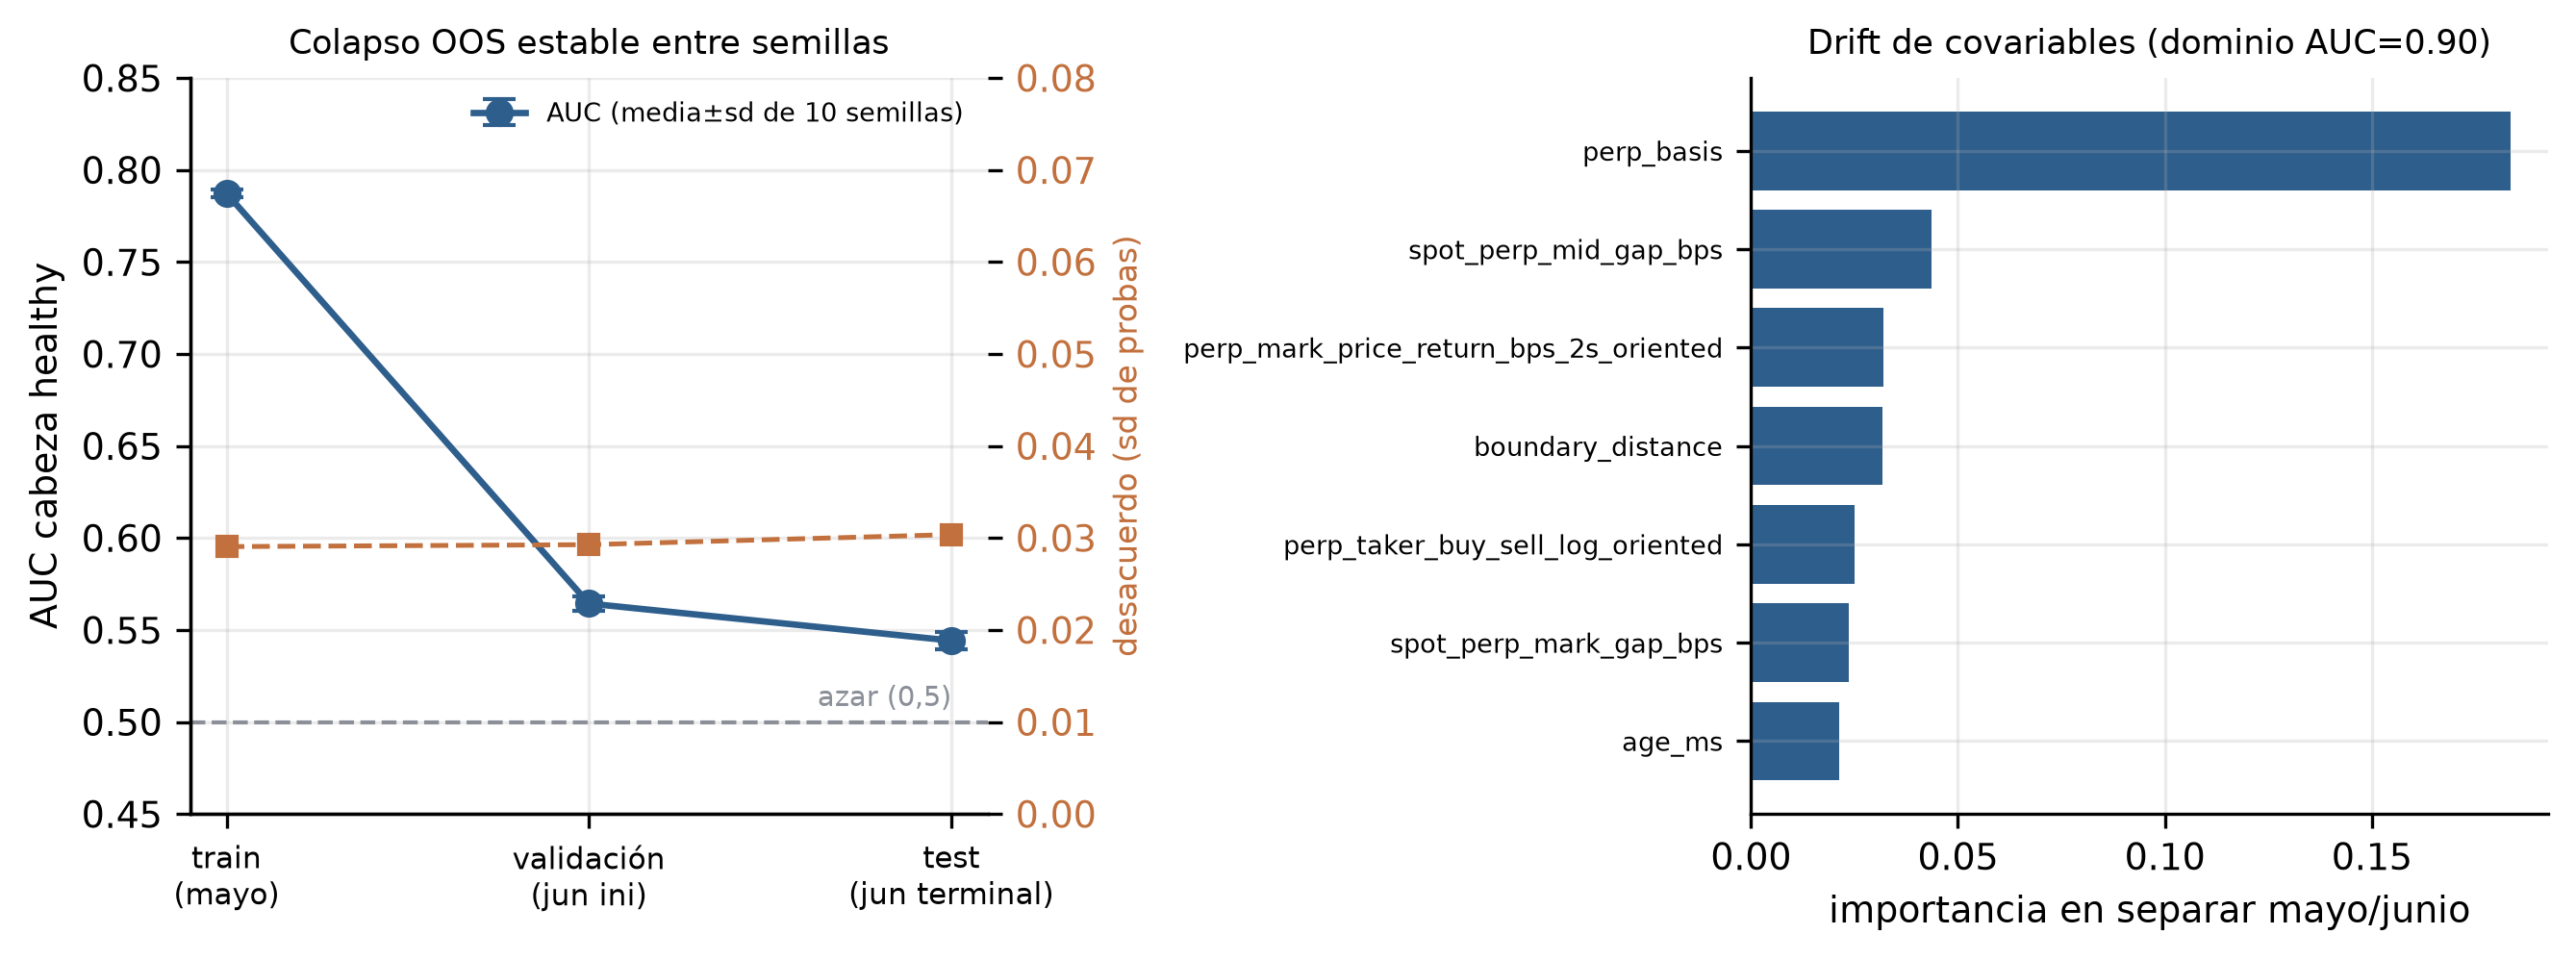
\includegraphics[width=\textwidth]{figures/fig_n3_ensemble_healthy.png}
\caption{Diagnóstico del fallo fuera de muestra de la cabeza de salud. Izquierda: el AUC
se desploma de entrenamiento a test con una dispersión mínima entre las diez réplicas
(barras de error) y un desacuerdo entre réplicas plano (línea naranja) —el fallo es
estable y no es epistémico. Derecha: un clasificador de dominio separa mayo de junio con
AUC $0{,}90$, señal de un fuerte desplazamiento de covariables encabezado por la base del
perpetuo.}
\label{fig::n3}
\end{figure}

\subsection{Curva de escalado de datos: tabular frente a aprendizaje profundo}
\label{sec::escalado_tab_deep}

La conclusión anterior —el tabular sencillo bate a la red profunda con pocos datos— invita
a una objeción natural: ¿no ganaría la vía profunda con más datos, dada su mayor capacidad?
Se responde empíricamente con una curva de escalado que enfrenta a ambas vías sobre la
\emph{misma} tarea y evaluación. Se predice la dirección del tramo H60 en los 906 casos
congelados a partir de ventanas de contexto régimen-ajustadas y sin fuga; la vía profunda
es el fine-tuning de MOMENT (Sección~\ref{sec::escalera}) y la tabular un \emph{gradient
boosting} sobre características clásicas derivadas de la misma ventana (retornos a varios
rezagos, momentum, volatilidad realizada y distancia a $0{,}5$). Ambas se entrenan sobre
subconjuntos crecientes del mismo corpus —de 3.000 a algo más de 41.000 ventanas— y se
evalúan sobre los mismos casos (Figura~\ref{fig::escalado_tab_deep}).

El resultado es inequívoco: la vía tabular domina a la profunda \emph{en todo el rango de
datos}. Con el corpus mínimo, la tabular acierta un 48,2\,\% frente al 46,0\,\% de
MOMENT; con el corpus completo, la tabular sube hasta el 50,3\,\% mientras que la
profunda se estanca en torno al 46,8\,\%. Es decir, la vía tabular no solo parte de un
nivel más alto, sino que además escala al menos tan bien: la brecha no se cierra al añadir
datos, se ensancha. La objeción queda respondida en negativo —al menos en este régimen de
tamaño de corpus— y refuerza la elección del modelo tabular como vehículo de la señal. La
lección para el proyecto es coherente con el resto del trabajo: la complejidad del modelo
no es el cuello de botella, de modo que no compra rendimiento; con dos semanas de datos, la
capacidad de una red profunda es una desventaja, no una ventaja.

\begin{figure}[htbp]
\centering
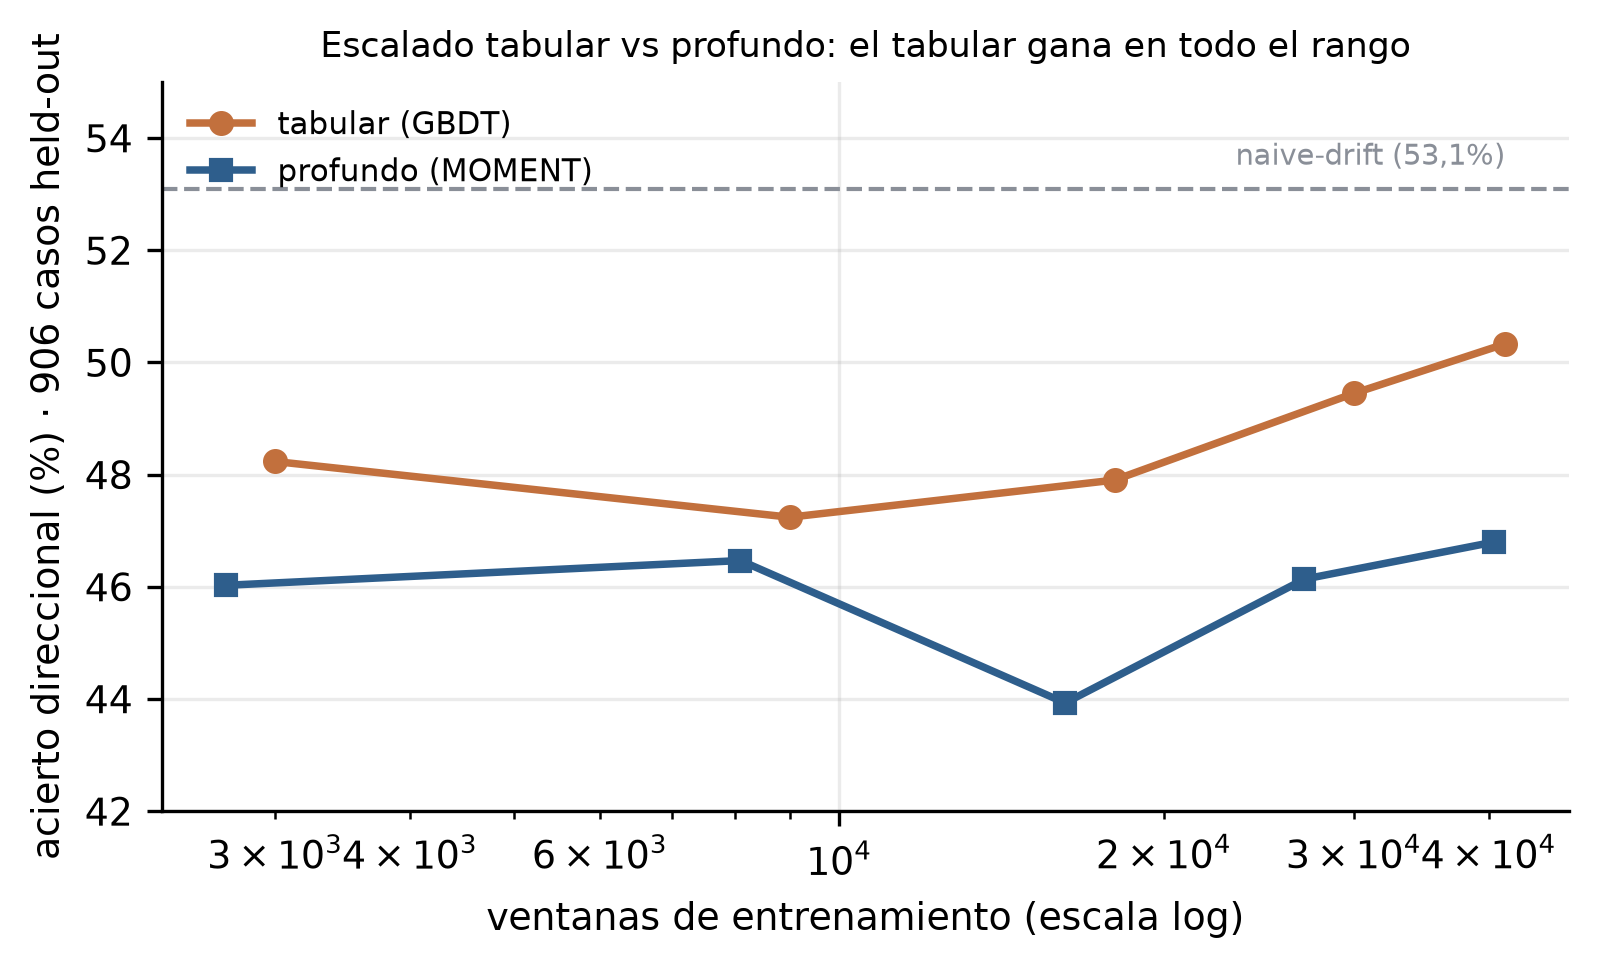
\includegraphics[width=0.72\textwidth]{figures/fig_scaling_tab_vs_deep.png}
\caption{Curva de escalado sobre la misma tarea (dirección H60, 906 casos congelados): la
vía tabular (\emph{gradient boosting}) supera a la profunda (MOMENT) en todo el presupuesto
de datos, y la distancia se mantiene o crece al aumentar el número de ventanas de
entrenamiento. Con este horizonte de datos, más muestras no hacen que el aprendizaje
profundo alcance al tabular.}
\label{fig::escalado_tab_deep}
\end{figure}
